%\documentclass[twoside, a4paper, draft]{article}
\documentclass[twoside, a4paper]{article}

%	A header file that makes it easy to produce common mathematical operations,
%	such as the partial derivatives, curl, div etc...

\newcommand{\gv}[1]{\ensuremath{\mbox{\boldmath$ #1 $}}} 			% for vectors of Greek letters
\newcommand{\uv}[1]{\ensuremath{\mathbf{\hat{#1}}}} 				% for unit vector
\newcommand{\abs}[1]{\left| #1 \right|} 							% for absolute value
\newcommand{\avg}[1]{\left< #1 \right>} 							% for average

\let\underdot=\d 													% rename builtin command \d{} to \underdot{}
\renewcommand{\d}[2]{\frac{d #1}{d #2}} 							% for derivatives
\newcommand{\dd}[2]{\frac{d^2 #1}{d #2^2}}							% for double derivatives
\newcommand{\pd}[2]{\frac{\partial #1}{\partial #2}} 				% for partial derivatives
\newcommand{\pdd}[2]{\frac{\partial^2 #1}{\partial #2^2}} 			% for double partial derivatives
\newcommand{\pDD}[3]{\frac{\partial^2 #1}{\partial #2 \partial #3}}			% for double partial derivative w.r.t different variables
\newcommand{\pdc}[3]{\left( \frac{\partial #1}{\partial #2} \right)_{#3}} % for thermodynamic partial derivatives

\newcommand{\ket}[1]{\left| #1 \right>} 							% for Dirac bras
\newcommand{\bra}[1]{\left< #1 \right|} 							% for Dirac kets
\newcommand{\braket}[2]{\left< #1 \vphantom{#2} \right| \left. #2 \vphantom{#1} \right>} % for Dirac brackets
\newcommand{\matrixel}[3]{\left< #1 \vphantom{#2#3} \right| #2 \left| #3 \vphantom{#1#2} \right>} % for Dirac matrix elements

\newcommand{\grad}[1]{\nabla #1} 				% for gradient
\let\divsymb=\div 									% rename builtin command \div to \divsymb
\renewcommand{\div}[1]{\nabla \cdot \gv{#1}} 		% for divergence
\newcommand{\curl}[1]{\nabla \times \gv{#1}} 		% for curl
\let\baraccent=\= 									% rename builtin command \= to \baraccent
\renewcommand{\=}[1]{\stackrel{#1}{=}} 				% for putting numbers above =

\newcommand{\curlv}[1]{\curl{\vec{ #1 }}}			% curl with a vector symbol
\newcommand{\divv}[1]{\div{\vec{#1}}}				% div of a vector
\newcommand{\pdv}[2]{\pd{\gv{#1}}{#2}}				% partial derivative with a vector symbol
\newcommand{\pddv}[2]{\pdd{\gv{#1}}{#2}}			% 2nd partial derivative of a vector

\usepackage{amsmath}
\usepackage{amssymb}
\usepackage{amsfonts}
\usepackage{verbatim}
\usepackage{cite}
\usepackage{setspace}
\usepackage{textcomp}
\usepackage{graphicx}
%\usepackage[dvips]{graphicx}

\title{Orthogonal Curvilinear Coordinate Differentiation Operators}
\author{Marko Milicevic}
\date{}	% Don't print the date
%\doublespacing
%\linespread{1.5}

\begin{document}
\maketitle

\begin{abstract}

In this chapter we derive the curvilinear representation of the grad, div, curl and Laplace operators. Such representations are useful in solving Maxwell's equations in various coordinate systems, most notably cylindrical and spherical coordinates.

\end{abstract}

\section{Curvilinear Coordinates}
Let the Cartesian coordinates $x,y,z$ of a point $P$ be given by the single-valued, differentiable functions

\begin{equation*}
x=f_x(q_1,q_2,q_3) \quad y=f_y(q_1,q_2,q_3) \quad z=f_z(q_1,q_2,q_3)
\end{equation*}

Each point in space is then uniquely determined by the values of $q_1, q_2,q_3$ which are called the `\textit{curvilinear coordinates}'.
If we set $q_i$ to be constant then a 2-dimensional surface is formed which we'll label $\Omega(q_i)$ (figure \ref{fig:q_surfaces}). If the surfaces of $\Omega(q_1)$, $\Omega(q_2)$ and $\Omega(q_3)$ intersect at a point $P$ then the curvilinear coordinates of $P$ are given as as $q_1, q_2, q_3$. We will restrict ourselves to \textit{orthogonal} coordinates in which  the 2-dimensional surfaces $\Omega$ always intersect at right angles with each other.\\

\begin{figure}[htbp]
	\centering
	\fbox{
	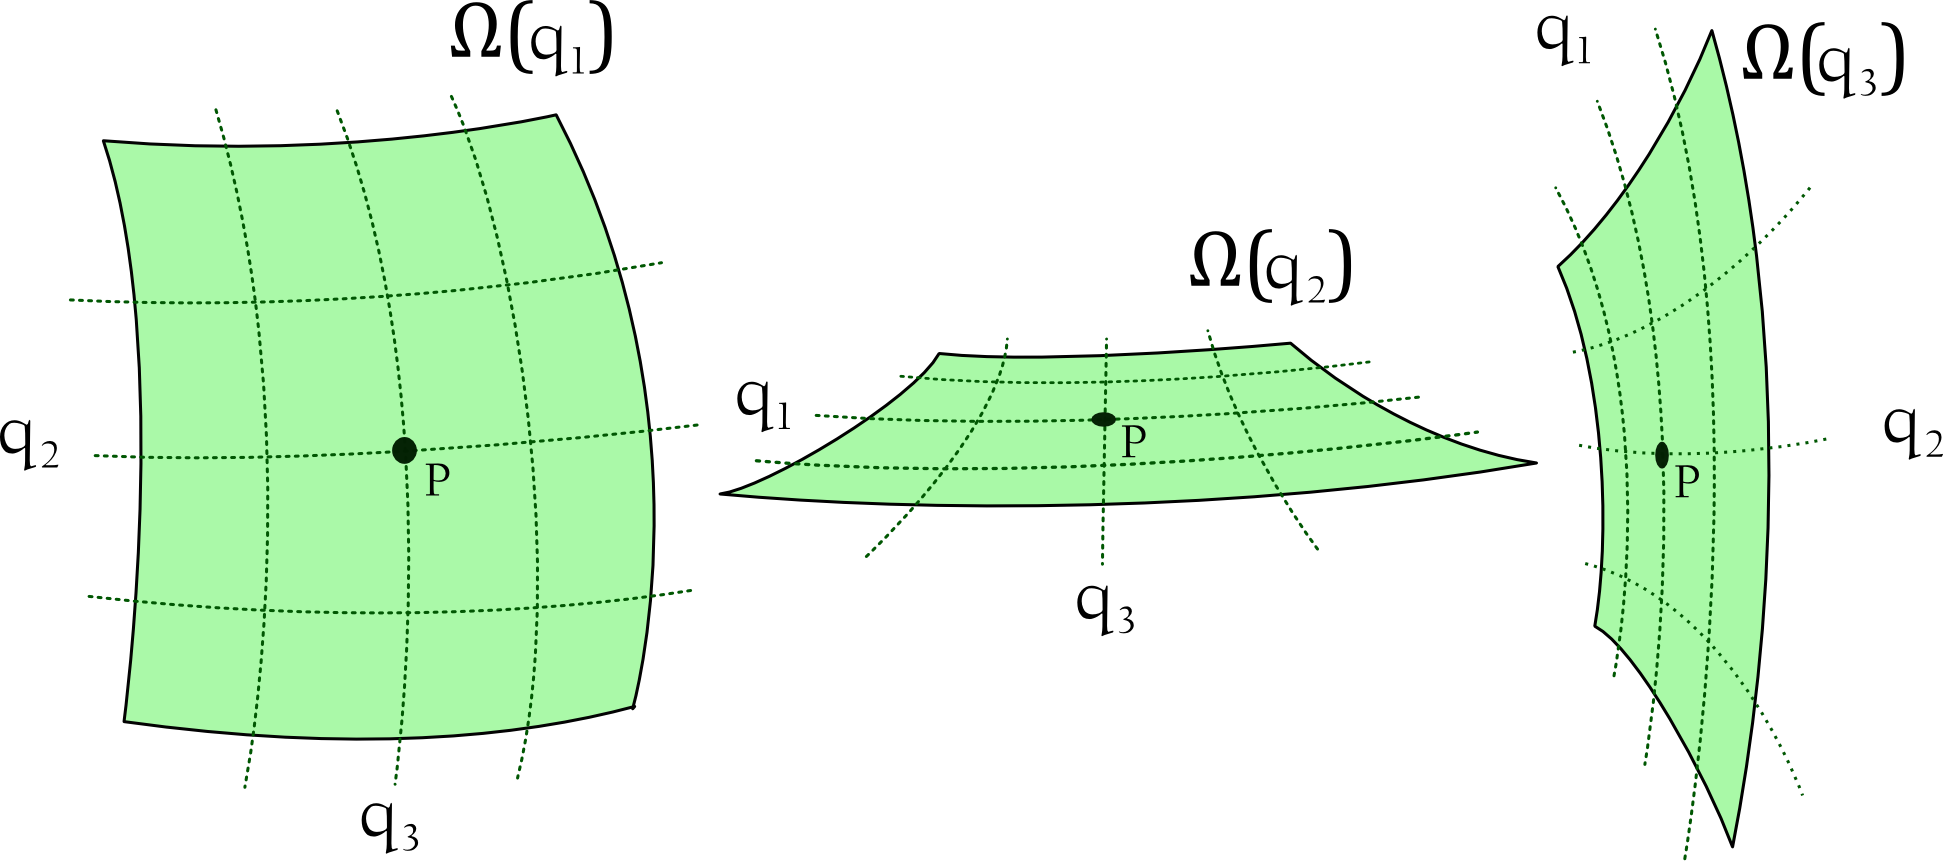
\includegraphics[width=115mm]{pic/curvilinear_coords_surfaces.png}
	}
	\caption{characteristic $\Omega$ surfaces obtained by setting $q_i$ to be constant}
	\label{fig:q_surfaces}
\end{figure}

In addition to specifying a point in space, $(q_1,q_2,q_3)$ can also be used to specify direction. We'll let $\uv{v}_i$ be the unit vector that points \textit{normal} to the surface $\Omega(q_i)$. A vector $\gv{F}$ can be expressed in this new basis as

\begin{equation*}
\gv{F} = F_1 \uv{v}_1 + F_2 \uv{v}_2 + F_3 \uv{v}_3
\end{equation*}

Since we're dealing with orthogonal coordinates $\uv{v}_i$ are mutually perpendicular, however unlike the Cartesian vectors $\uv{i}, \uv{j}, \uv{k}$ the directions specified by $\uv{v}_1, \uv{v}_2, \uv{v}_3$ may vary in space.\\

Since $q_1, q_2, q_3$ won't necessarily represent distances a metric is needed to determine the displacement $d\gv{s}$ between points \hbox{$(q_1,q_2,q_3)$} and \mbox{$(q_1+dq_1,q_2+dq_2,q_3+dq_3)$}.
\begin{equation}
\label{eq:ds_vector}
d\gv{s} = h_1 dq_1 \uv{v}_1 + h_2 dq_2 \uv{v}_2 + h_3 dq_3 \uv{v}_3
\end{equation}
Where the quantities $h_i$ are in general functions of $q_1,q_2,q_3$.

\section{Gradient}

The change in a scalar function $f(q_1,q_2,q_3)$ is given by 

\begin{equation}
\label{eq:df}
df = \pd{f}{q_1}dq_1+\pd{f}{q_2}dq_2+\pd{f}{q_3}dq_3
\end{equation}

It's gradient $\nabla f$ is defined by

\begin{equation}
\label{eq:grad}
df = \nabla f \cdot d\gv{s}
\end{equation}

Substituting equation (\ref{eq:ds_vector}) into (\ref{eq:grad})

\begin{equation}
\label{eq:df-dot-ds}
\begin{split}
df 
& = \nabla f \cdot 
	\Big( h_1 dq_1 \uv{v}_1 + h_2 dq_2 \uv{v}_2 + h_3 dq_3 \uv{v}_3 \Big) \\
& = \Big( \left( \nabla f \right)_1 \uv{v}_1 + \left( \nabla f \right)_2 \uv{v}_2 + \left( \nabla f \right)_3 \uv{v}_3 \Big) \cdot 
	\Big( h_1 dq_1 \uv{v}_1 + h_2 dq_2 \uv{v}_2 + h_3 dq_3 \uv{v}_3 \Big) \\
& = \left( \nabla f \right)_1 h_1 dq_1 + 
	 \left( \nabla f \right)_2 h_2 dq_2 + 
	 \left( \nabla f \right)_3 h_3 dq_3 \\
\end{split}
\end{equation}

Comparing (\ref{eq:df-dot-ds}) with (\ref{eq:df}) and equating the coefficients of each $dq_i$ gives

\begin{equation}
\label{eq:grad_f}
\boxed{
\nabla f = \frac{1}{h_1} \pd{f}{q_1} \uv{v}_1 + \frac{1}{h_2} \pd{f}{q_2} \uv{v}_2 + \frac{1}{h_3} \pd{f}{q_3} \uv{v}_3
}
\end{equation}

\section{Divergence}
To find the curvilinear expression for divergence we make use of Gauss's theorem

\begin{equation}
\label{eq:divergence_theorem}
\int_{\partial V} \gv{F} \cdot d\gv{A} = \int_{V} \div{F} \: dV
\end{equation}

Where the left hand side of (\ref{eq:divergence_theorem}) is a surface integral over a boundary $\partial V$ and the right hand side is a volume integral enclosed by the boundary. By focusing in on an infinitesimal volume element centred about $q_1,q_2,q_3$ we can rewrite (\ref{eq:divergence_theorem}) as

\begin{align*}
\lim_{\int dV \to 0} \int \gv{F} \cdot d\gv{A} = &
\lim_{\int dV \to 0} \int \div{F} \: dV \\
= & \div{F}(q_1,q_2,q_3) \lim_{\int dV \to 0} \int dV \\
\end{align*}
\begin{equation}
\label{eq:divergence_theorem_limit}
\Rightarrow 
\boxed{
\displaystyle \div{F} = \lim_{\int dV \to 0}\frac{ \int_{\partial V} \gv{F} \cdot d\gv{A} }{ \int dV }
}
\end{equation}

Figure \ref{fig:divergence} shows an infinitesimal region with the bounding curves $\Omega(q_1)$ and $\Omega(q_1+dq_1)$ shaded.

\begin{figure}[htbp]
	\centering
	\fbox{
	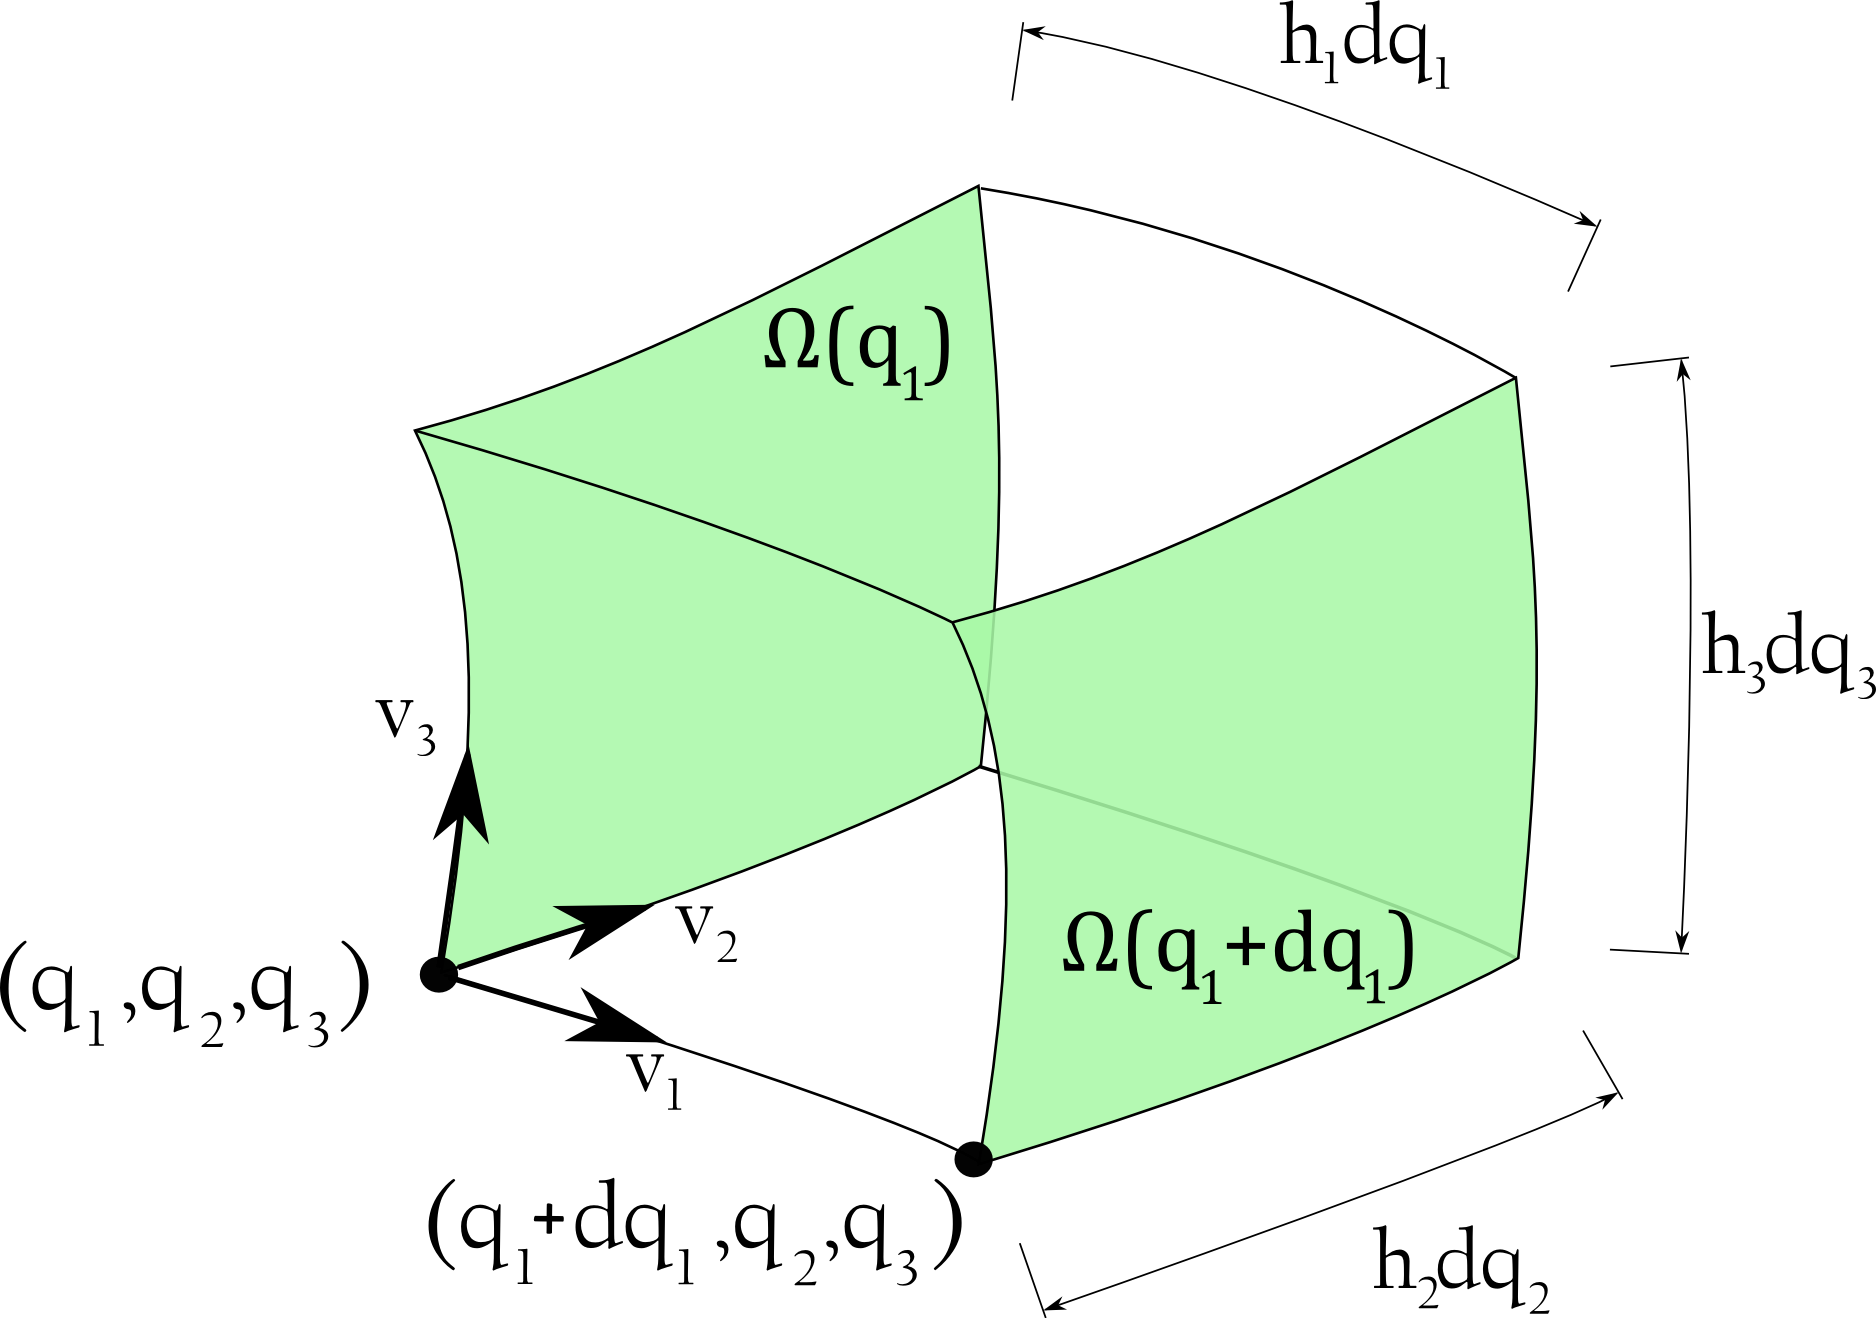
\includegraphics[width=110mm]{pic/curvilinear_coords_div2.png}
	}
	\caption{Infinitesimal parallelepiped with the bounding planes $\Omega(q_1)$ and \mbox{$\Omega(q_1+dq_1)$} highlighted}
	\label{fig:divergence}
\end{figure}

The flux $\int \gv{F} \cdot d\gv{A}$ through these shaded surfaces is

\begin{align*}
\int_{\Omega(q_1)} \gv{F} \cdot d\gv{A}	 & = \gv{F}(q_1,q_2,q_3) \cdot d\gv{A} \\
		 & = \gv{F} \cdot (-\uv{v}_1 \, dA) \\
		 & = -F_1 h_2 h_3 dq_2 dq_3
\end{align*}
\begin{align*}
\int_{\Omega(q_1+dq_1)} \gv{F} \cdot d\gv{A} & = \gv{F} (q_1+dq_1,q_2,q_3) \cdot d\gv{A} \\
	 & = \gv{F} (q_1+dq_1,q_2,q_3) \cdot (\uv{v}_1 \, dA) \\
	 & = F_1(q_1+dq_1,q_2,q_3) h_2(q_1+dq_1,q_2,q_3) h_3(q_1+dq_1,q_2,q_3) dq_2 dq_3 \\
	 & = \Big[ F_1 h_2 h_3 + \frac{\partial}{\partial q_1} \big( F_1 h_2 h_3 \big) dq_1 \Big] dq_2 dq_3
\end{align*}

Where quantities are evaluated at $q_1,q_2,q_3$ unless otherwise stated.
The net flux through the shaded regions is thus

\begin{align*}
\int_{\Omega(q_1+dq_1)} + \int_{\Omega(q_1)} & = \Big[ \frac{\partial}{\partial q_1} \big( F_1 h_2 h_3 \big) dq_1 \Big] dq_2 dq_3
\end{align*}

Likewise a similar argument applies to the flux calculated through the $\Omega(q_2)$, $\Omega(q_2+dq_2)$ and the $\Omega(q_3)$, $\Omega(q_3+dq_3)$ surfaces and the result can be obtained by cyclically permutating the $q_1, q_2, q_3$ coordinates

\begin{align*}
\int_{\Omega(q_2+dq_2)} + \int_{\Omega(q_2)} & = \Big[ \frac{\partial}{\partial q_2} \big( F_2 h_1 h_3 \big) \Big] dq_1 dq_2 dq_3 \\
\int_{\Omega(q_3+dq_3)} + \int_{\Omega(q_3)} & = \Big[ \frac{\partial}{\partial q_3} \big( F_3 h_1 h_2 \big) \Big] dq_1 dq_2 dq_3
\end{align*}

Finally we obtain the total flux through an infinitesimal parallelepiped to be the sum over all these surfaces

\begin{equation}
\label{eq:flux}
\begin{split}
\int \gv{F} \cdot d\gv{A} = &  
\Big[
\frac{\partial}{\partial q_1} \big( F_1 h_2 h_3 \big) + 
\frac{\partial}{\partial q_2} \big( F_2 h_1 h_3 \big) + 
\frac{\partial}{\partial q_3} \big( F_3 h_1 h_2 \big)
\Big] dq_1 dq_2 dq_3
\end{split}
\end{equation}

Substituting (\ref{eq:flux}) in (\ref{eq:divergence_theorem_limit}) and identifying the volume element $dV = h_1 h_2 h_3 dq_1 dq_2 dq_3$ gives

\begin{equation}
\label{eq:div}
\boxed{
\div{F} =
\frac{1}{h_1 h_2 h_3} 
\Big[
\frac{\partial}{\partial q_1} \big( F_1 h_2 h_3 \big) + 
\frac{\partial}{\partial q_2} \big( F_2 h_1 h_3 \big) + 
\frac{\partial}{\partial q_3} \big( F_3 h_1 h_2 \big) 
\Big]
}
\end{equation}

\section{Curl}

Stokes's theorem is employed to find the curvilinear curl operator

\begin{equation}
\label{eq:stoke-thm}
\int_{A} \curl{F} \cdot d\gv{A} = \int_{\partial A} \gv{F} \cdot d\gv{s}
\end{equation}

Where $A$ represents a 2-dimensional surface area and $\partial A$ it's boundary. Looking at an infinitesimal area element in the $\uv{v}_1, \uv{v}_2$ plane (see figure \ref{fig:curl}), the left hand side of (\ref{eq:stoke-thm}) becomes

\begin{equation}
\label{eq:stokes-lhs}
\begin{split}
\curl{F} \cdot d\gv{A} & = \curl{F} \cdot dA \uv{v}_3 \\
& = \big[ \curl{F} \big]_3 \: dA \\
& = \big[ \curl{F} \big]_3 \: h_1 h_2 \: dq_1 dq_2
\end{split}
\end{equation}

\begin{figure}[htbp]
	\centering
	\fbox{
	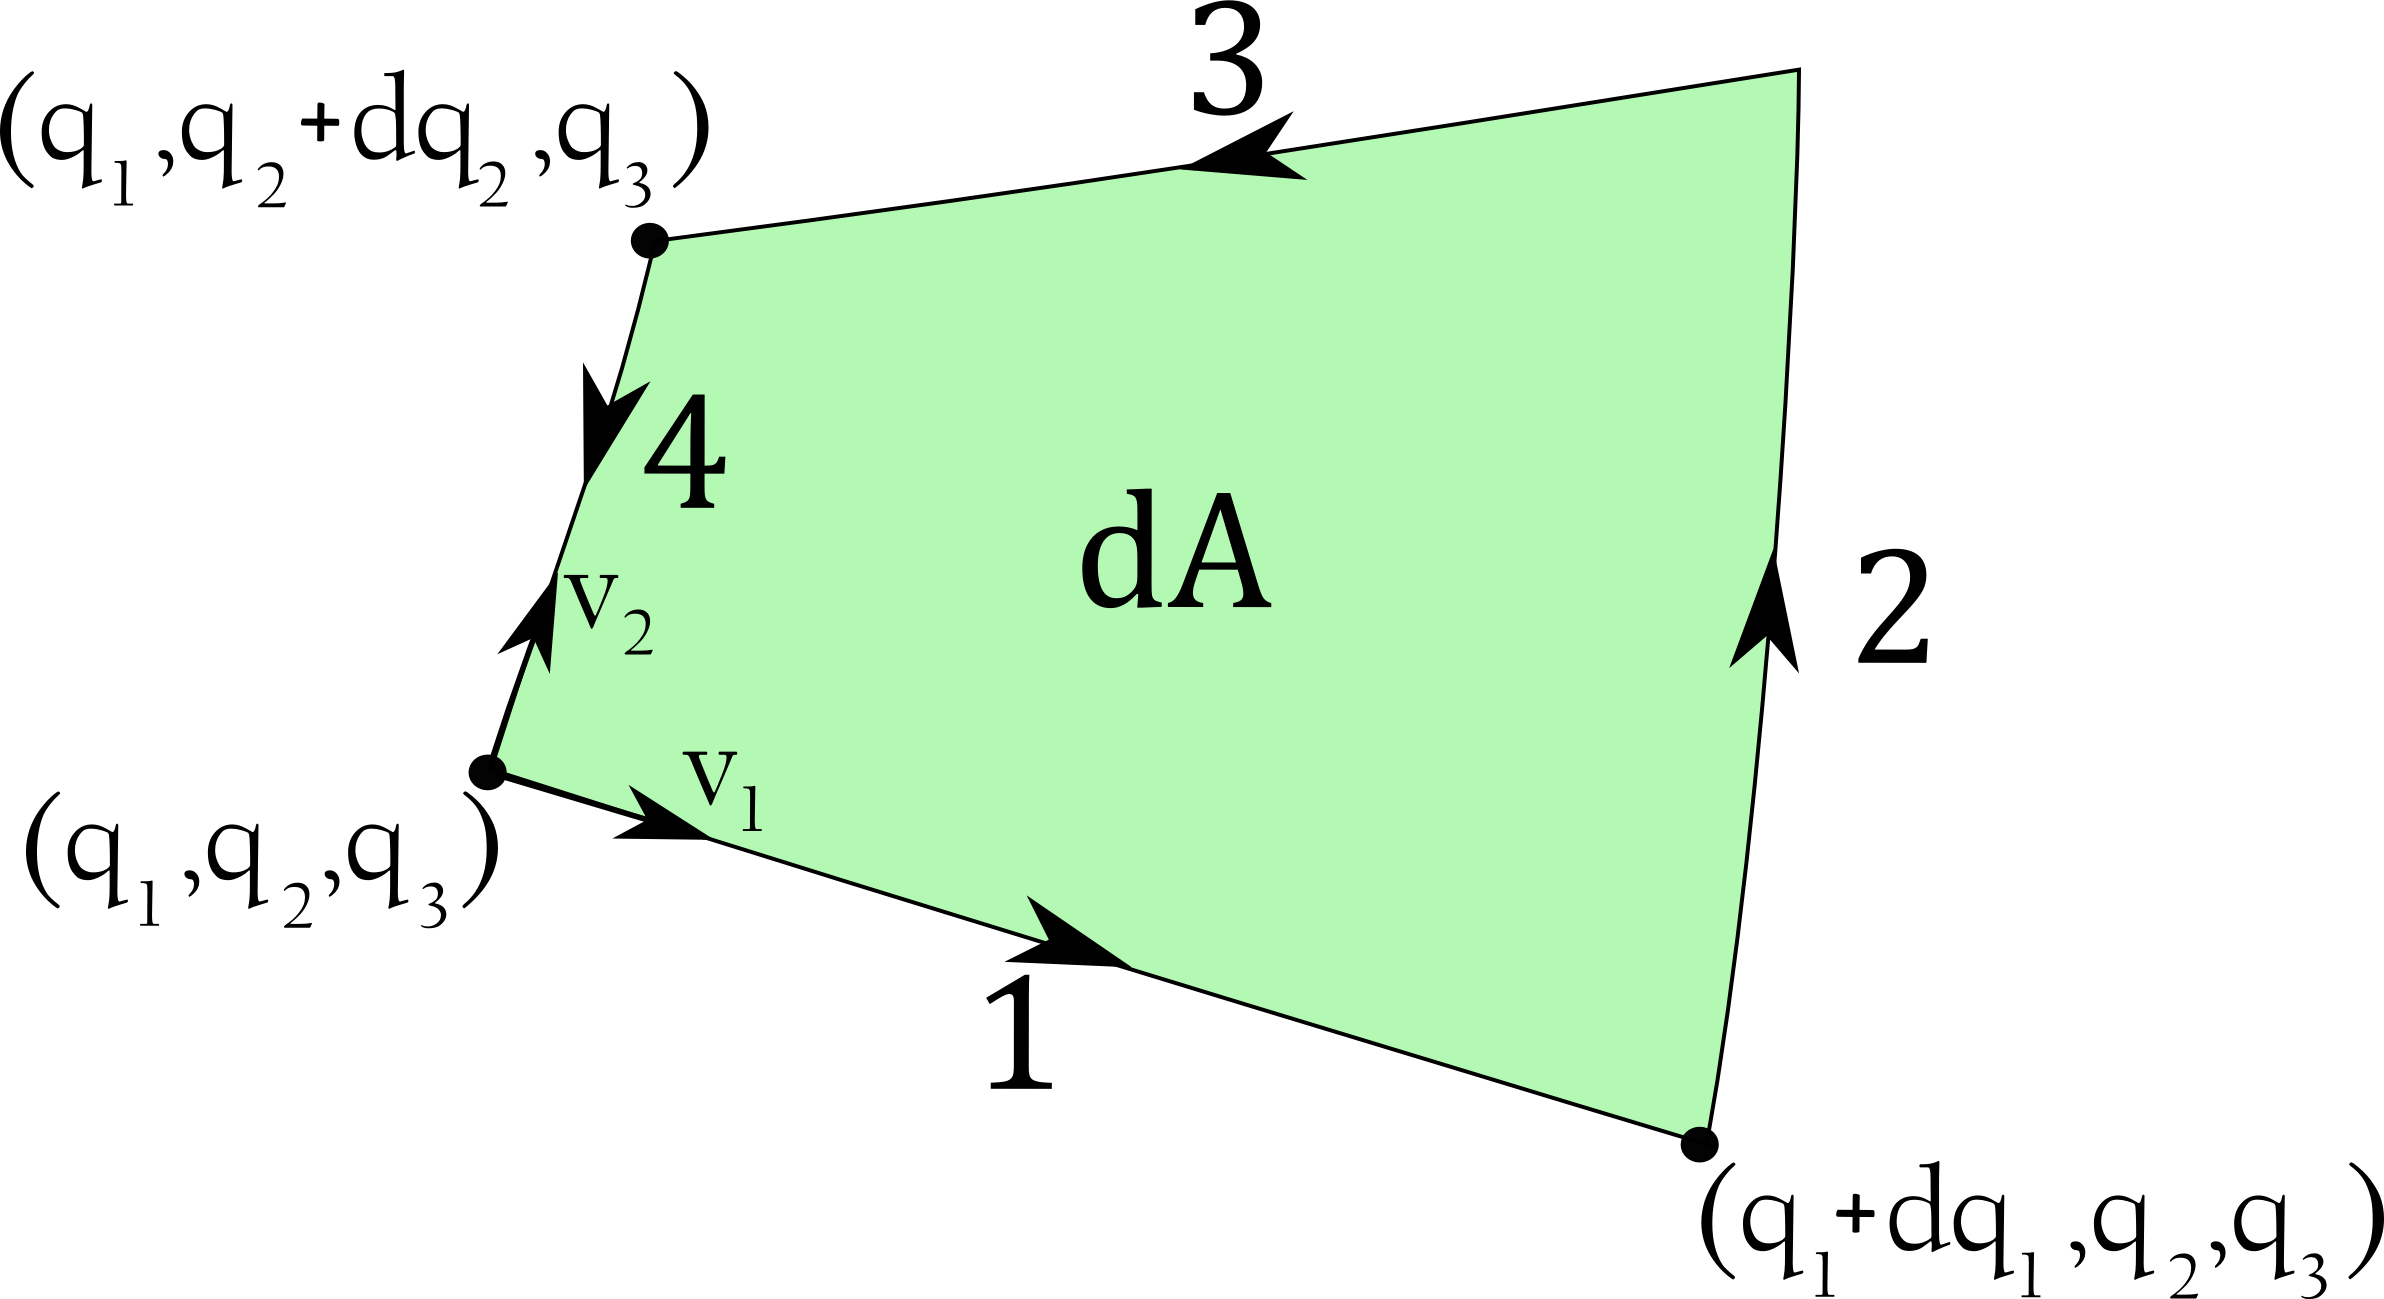
\includegraphics[width=110mm]{pic/curvilinear_coords_curl.png}
	}
	\caption{An infinitesimal area element in the $\uv{v}_1,\uv{v}_2$ plane, $\uv{v}_3$ is directed out of the page}
	\label{fig:curl}
\end{figure}

The line integral $\int \gv{F} \cdot d\gv{s}$ is calculated in 4 different parts, with paths labelled 1-4 in figure \ref{fig:curl}. 

\begin{align*}
\int_{\partial A} \gv{F} \cdot d\gv{s} & = 
\bigg( 
\int_1 + \int_2 + \int_3 + \int_4 
\bigg)
\gv{F} \cdot d\gv{s} \\
\int_1 \gv{F} \cdot d\gv{s}
& = \gv{F} \cdot \left( h_1 \, dq_1 \, \uv{v}_1 \right) \\
& = F_1 \, h_1 \, dq_1 \\
\int_2 \gv{F} \cdot d\gv{s}
& = \gv{F}(q_1+dq_1, q_2) \cdot \left( h_2(q_1+dq_1, q_2) \, dq_2 \, \uv{v}_2 \right) \\
& = F_2(q_1+dq_1, q_2) \, h_2(q_1+dq_1, q_2) \, dq_2 \\
& = \Big[ F_2 \, h_2 + \pd{}{q_1} \left( F_2 \, h_2 \right) dq_1 \Big] dq_2 \\
\int_3 \gv{F} \cdot d\gv{s}
& = \gv{F}(q_1, q_2+dq_2) \cdot \left( h_1(q_1, q_2+dq_2) \, dq_1 \, (-\uv{v}_1) \right) \\
& = -F_1(q_1, q_2+dq_2) \, h_1(q_1, q_2+dq_2) \, dq_1 \\
& = -\Big[ F_1 \, h_1 + \pd{}{q_2} \left( F_1 \, h_1 \right) dq_2 \Big] dq_1 \\
\int_4 \gv{F} \cdot d\gv{s}
& = \gv{F} \cdot \left( h_2 \, dq_2 \, (-\uv{v}_2) \right) \\
& = -F_2 \, h_2 \, dq_2
\end{align*}

Summing up all the paths of the line integral

\begin{equation}
\label{eq:stokes-rhs}
\int_{\partial A} \gv{F} \cdot d\gv{s}
=
\bigg[
\pd{}{q_1} \left( F_2 h_2 \right) - \pd{}{q_2} \left( F_1 h_1 \right)
\bigg]
dq_1 \, dq_2
\end{equation}

Substituting (\ref{eq:stokes-lhs}) and (\ref{eq:stokes-rhs}) into (\ref{eq:stoke-thm})

\begin{equation*}
\big[ \curl{F} \big]_3 = 
\frac{1}{h_1 h_2}
\bigg[
\pd{}{q_1} \left( F_2 h_2 \right) - \pd{}{q_2} \left( F_1 h_1 \right)
\bigg]
\end{equation*}

Derivations for the other components of $\curl{F}$ are identical to the above with cyclical permutations of $(1,2,3)$.

\begin{equation}
\label{eq:curl-components}
\begin{split}
\big[ \curl{F} \big]_1 = 
\frac{1}{h_2 h_3}
\bigg[
\pd{}{q_2} \left( F_3 h_3 \right) - \pd{}{q_3} \left( F_2 h_2 \right)
\bigg] \\
\big[ \curl{F} \big]_2 = 
\frac{1}{h_1 h_3}
\bigg[
\pd{}{q_3} \left( F_1 h_1 \right) - \pd{}{q_1} \left( F_3 h_3 \right)
\bigg] \\
\big[ \curl{F} \big]_3 = 
\frac{1}{h_1 h_2}
\bigg[
\pd{}{q_1} \left( F_2 h_2 \right) - \pd{}{q_2} \left( F_1 h_1 \right)
\bigg]
\end{split}
\end{equation}

Equations (\ref{eq:curl-components}) can be summarised in the form

\begin{equation}
\label{eq:curl}
\boxed{
\displaystyle
\curl{F} = 
\frac{1}{h_1 \, h_2 \, h_3}
\begin{vmatrix}
h_1 \, \uv{v}_1	&		h_2 \, \uv{v}_2		&		h_3 \, \uv{v}_3 \\
 & & \\
\displaystyle \pd{}{q_1}	&	\displaystyle \pd{}{q_2}	&	\displaystyle \pd{}{q_3} \\
 & & \\
F_1 \, h_1		&		F_2 \, h_2		&		F_3 \, h_3
\end{vmatrix}
}
\end{equation}

\section{Laplace operator}

The Laplace operator $\nabla^2$ acting on a scalar $f$ is defined as

\begin{equation}
\label{eq:laplace-definition}
\nabla^2 f = \gv{\nabla} \cdot \left( \gv{\nabla} f \right)
\end{equation}

Substituting the curvilinear definitions for the gradient (\ref{eq:grad_f}) and divergence (\ref{eq:div}) into (\ref{eq:laplace-definition}) results in the curvilinear Laplace operator expression

\begin{equation}
\label{eq:laplace}
\boxed{
\begin{split}
\nabla^2 f = & 
\frac{1}{h_1 \, h_2 \, h_3}
\bigg[
\pd{}{q_1} \left( \frac{h_2 \, h_3}{h_1} \pd{f}{q_1} \right) \\
& \quad \quad \quad \quad \quad
+ \pd{}{q_2} \left( \frac{h_1 \, h_3}{h_2} \pd{f}{q_2} \right) +
\pd{}{q_3} \left( \frac{h_1 \, h_2}{h_3} \pd{f}{q_3} \right)
\bigg]
\end{split}
}
\end{equation}

\end{document}
